
\documentclass[12pt]{amsart}
\usepackage{geometry} % see geometry.pdf on how to lay out the page. There's lots.
\geometry{a4paper} % or letter or a5paper or ... etc
\usepackage[T1]{fontenc}
\usepackage[latin9]{inputenc}
\usepackage{amsmath}
\usepackage{amsaddr}
\usepackage{dirtytalk}
\usepackage{float}
\usepackage{listings}
\usepackage{hyperref}
\usepackage{enumerate}
\usepackage{graphicx}

\usepackage{color}
 
\definecolor{codegreen}{rgb}{0,0.6,0}
\definecolor{codegray}{rgb}{0.5,0.5,0.5}
\definecolor{stringcolor}{rgb}{0.7,0.23,0.36}
\definecolor{backcolour}{rgb}{0.95,0.95,0.92}
\definecolor{keycolor}{rgb}{0.007,0.01,1.0}
\definecolor{itemcolor}{rgb}{0.01,0.0,0.49}

\hypersetup{
    colorlinks=true,
    linkcolor=blue,
    filecolor=blue,      
    urlcolor=blue,
}
 
\lstdefinestyle{mystyle}{
    %backgroundcolor=\color{backcolour},   
    commentstyle=\color{codegreen},
    keywordstyle=\color{keycolor},
    numberstyle=\tiny\color{codegray},
    stringstyle=\color{stringcolor},
    basicstyle=\footnotesize,
    breakatwhitespace=false,         
    breaklines=true,                 
    captionpos=b,                    
    keepspaces=true,                 
    numbers=left,                    
    numbersep=5pt,                  
    showspaces=false,                
    showstringspaces=false,
    showtabs=false,                  
    tabsize=2
}
 
\lstset{style=mystyle}

\lstdefinelanguage{Swift}{
  keywords={associatedtype, class, deinit, enum, extension, func, import, init, inout, internal, let, operator, private, protocol, public, static, struct, subscript, typealias, var, break, case, continue, default, defer, do, else, fallthrough, for, guard, if, in, repeat, return, switch, where, while, as, catch, dynamicType, false, is, nil, rethrows, super, self, Self, throw, throws, true, try, associativity, convenience, dynamic, didSet, final, get, infix, indirect, lazy, left, mutating, none, nonmutating, optional, override, postfix, precedence, prefix, Protocol, required, right, set, Type, unowned, weak, willSet},
  ndkeywords={class, export, boolean, throw, implements, import, this},
  sensitive=false,
  comment=[l]{//},
  morecomment=[s]{/*}{*/},
  morestring=[b]',
  morestring=[b]"
}

\lstset{emph={Int,count,abs,repeating,Array}, emphstyle=\color{itemcolor}}


\title{Week 10}

\date{\today}

\lstset{style=mystyle}

%%% BEGIN DOCUMENT
\begin{document}
\maketitle

\section{Preparation for Assignment}
If, and \textit{only if} you can truthfully assert the truthfulness of each statement below are you ready to start the exercises.
\subsection {Reading Comprehension Self-Check}
\begin{itemize}
\item I know that the iterative-improvement technique involves finding a solution to an optimization problem by generating a sequence of feasible solutions with improving values of the problem\textquoteright s objective function.
\item I know that each subsequent solution in such a sequence typically involves a small, localized change in the previous feasible solution.
\item I know that when no such change improves the value of the objective function, the algorithm returns the last feasible solution as optimal and stops.
\item I know that important problems that can be solved exactly by iterative-improvement algorithms include linear programming, maximizing the flow in a network, and matching the maximum possible number of vertices in a graph.
\item I know that the simplex method is the classic method for solving the general linear programming problem, and that it works by generating a sequence of adjacent extreme points of the problem\textquoteright s feasible region with improving values of the objective function.
\item I know that the maximum-flow problem asks to find the maximum flow possible in a network, a weighted directed graph with a source and a sink.
\item I know that a maximum cardinality matching is the largest subset of edges in a graph such that no two edges share the same vertex, and that for a bipartite graph, it can be found by a sequence of augmentations of previously obtained matchings.
\item I know that the stable marriage problem is to find a stable matching for elements of two n-element sets based on given matching preferences.
\item I know that the stable marriage problem always has a solution that can be found by the Gale-Shapley algorithm.

\end{itemize}
\subsection{Memory Self-Check}
What are the three types of iterative improvement discussed in Chapter 10? How are they similar and how are they different?
 \section{Week 10 Exercises}
\subsection{ Exercise 2 on page 359}
\subsection{Exercise 2 on page 371} 
\subsection{Exercise 1 on page 378} 


\section{Week 10 Problems}
\subsection{Not in the Book}
Consider the tiny section of a production line for a factory your see in Figure \ref{fig:factory1}. 
\begin{figure}[htb]
  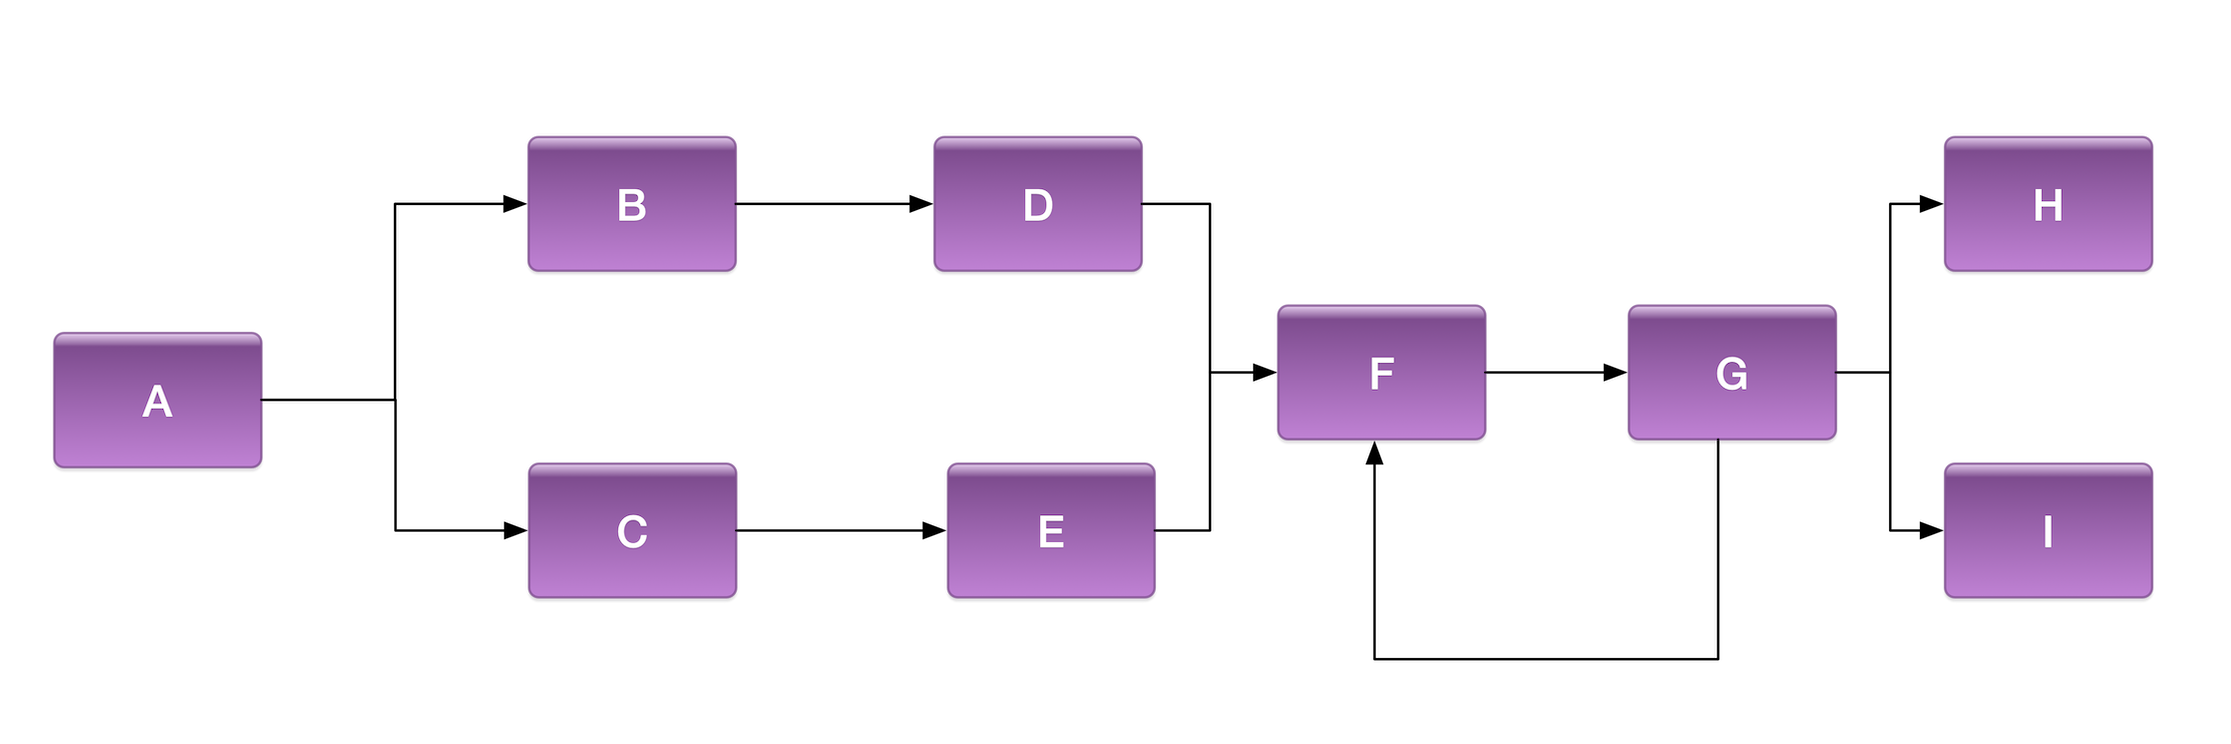
\includegraphics[width=\linewidth]{../support_files/tiny_factory.png}
  \caption{A Digraph of the Section of the Production Line.}
  \label{fig:factory1}
\end{figure}

\href{run:../support_files/tiny_factory_step_descriptions.pdff}{This pdf file} contains further descriptions of the factory.

Your task is to maximize the throughput of of this portion of the factory over a time span of 2000 units of time.

You are required to start with a baseline that always uses Same Type as the Selection Option for work to do. Then, apply an iterative improvement technique of your choice to improve throughput.

This problem requires creativity on your part. There are many ways to crunch these numbers and find solutions. 

 From \textit{How Mathematicians Think} by William Byers

\say{One of the aspects of a living system is that it is creative. Life is continually being confronted with problems and the necessity to resolve these problems. Problems, in life, in art, and in science, are inevitable. Not only can they not be avoided but they are the very things that spur development, that spur evolution. The solutions that these problematic situations bring forth are unpredictable, a priori. The solution to such problems often involves an element that is entirely unexpected --- the creative element. A creative solution is not mechanical --- it does not involve juggling a number of predetermined elements according to predetermined rules. It involves the emergence of a novel way of looking at the original situation. This new way of seeing is often generated by very incompatible tendencies within the original situation that made it problematic in the first place. This is the essence of a living system as it is the essence of mathematics --- nontrivial, creative, and alive.}




  


\end{document}